\documentclass[tikz,border=5mm,12pt]{standalone}
\usepackage[fontsize=16pt]{fontsize}
\usetikzlibrary{arrows.meta}

\newcommand\myfbox[1]{\fbox{#1\strut}}

\def\labelYsep{32pt}
\def\xsep{40mm}
\def\ysep{12mm}
\begin{document}
  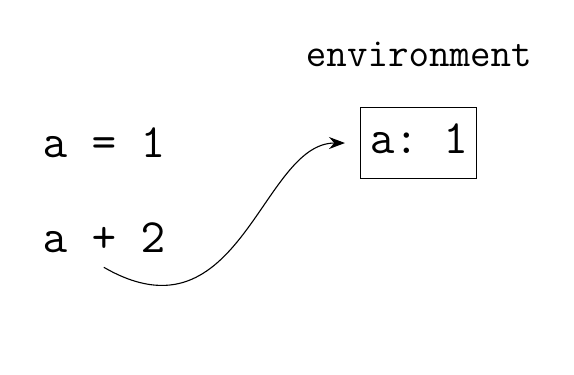
\begin{tikzpicture}[
    arrowtip/.style={
      -{Stealth[scale=1.2]}
    },
    curved/.style={
      in control={+(180:20mm)},
      out control={+(-30:20mm)}
    }
  ]
    \node at (0*\xsep, 0*\ysep) { \texttt{a\ =\ 1} };
    \node (OpB) at (0*\xsep,-1*\ysep) { \texttt{a\ +\ 2} };

    \node at (1*\xsep, \labelYsep) { \small\texttt{environment} };

    \node (EnvA) at (1*\xsep, 0*\ysep) { \myfbox{\texttt{a:\ 1}} };

    \draw[arrowtip,curved] (OpB.south) to (EnvA);
  \end{tikzpicture}
\end{document}
